\section{Proyecto lab08}
\begin{itemize}
  \item Creamos un directorio en fase02 que contenga los archivos del laboratorio
  \item Copiamos los archivos del anterior laboratorio
  \item Dejamos la clase Soldado.java igual por que cumple con los requisitos indicados en la actividad
  \item Para el tablero se usara un array bidimensional simple
\end{itemize}
La estructura final del laboratorio es: 
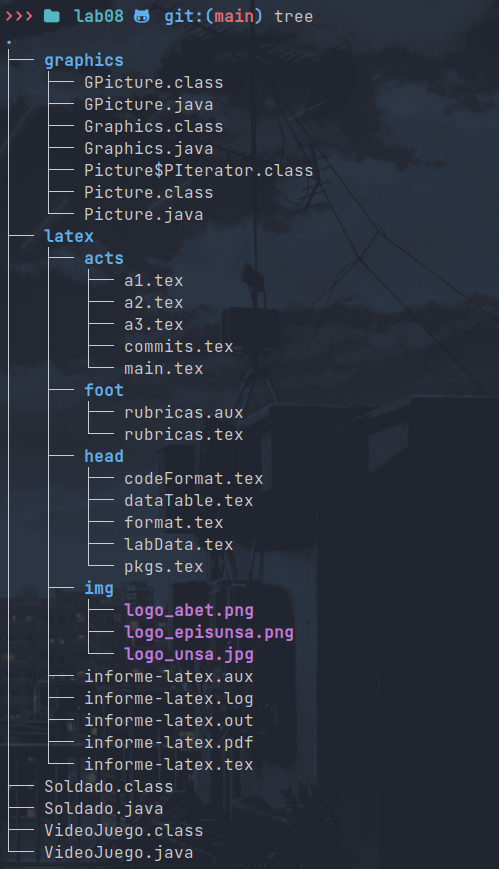
\includegraphics[width=0.3\textwidth]{img/tree.jpg}
